\documentclass[fleqn,12pt]{article}

\usepackage[margin=15mm]{geometry}
\usepackage[utf8]{inputenc}
\usepackage[bulgarian]{babel}
\usepackage[unicode]{hyperref}
\usepackage{amsfonts}
\usepackage{amssymb}
\usepackage{enumitem, hyperref}
\usepackage{upgreek}
\usepackage{indentfirst}
\usepackage{graphicx}
\usepackage{mathtools}

\usepackage[dvipsnames]{xcolor}

\usepackage{listings}
\usepackage{xcolor}

\graphicspath{ {./img/} }

\definecolor{codegreen}{rgb}{0,0.6,0}
\definecolor{codegray}{rgb}{0.5,0.5,0.5}
\definecolor{codepurple}{rgb}{0.58,0,0.82}
\definecolor{backcolour}{rgb}{0.95,0.95,0.92}

\lstdefinestyle{mystyle}{
    backgroundcolor=\color{backcolour},   
    commentstyle=\color{codegreen},
    keywordstyle=\color{magenta},
    numberstyle=\tiny\color{codegray},
    stringstyle=\color{codepurple},
    basicstyle=\ttfamily\footnotesize,
    breakatwhitespace=false,         
    breaklines=true,                 
    captionpos=b,                    
    keepspaces=true,                 
    numbers=left,                    
    numbersep=5pt,                  
    showspaces=false,                
    showstringspaces=false,
    showtabs=false,                  
    tabsize=2
}
\lstset{style=mystyle}


\title{Процедурно програмиране - основни информационни и алгоритмични структури (на базата на C++)}
\author{v1.0}
\date{23 юни 2021}

\begin{document}

\maketitle

\tableofcontents
\pagebreak

\section{Скаларни типове от данни}

\noindent \textit{\textbf{Деф}} - Тип данни наричаме \textbf{скаларен} ако той се състои само от една компонента, т.е. е атомарен. Например числови и булеви типове. \\
\noindent \textit{\textbf{Деф}} - Тип данни наричаме \textbf{съставен} ако той се състои от много компоненти. Например масиви. \\
\noindent \textit{\textbf{Деф}} - Тип данни наричаме \textbf{примитивен} когато той директно съдържа стойността. \\
\noindent \textit{\textbf{Деф}} - Тип данни наричаме \textbf{указател} ако той съдържа адреса към локацията в паметта където се пази стойността. \\

\subsection{Целочислени типове}

\subsubsection{Определение}
\noindent \textit{\textbf{Деф}} - Целочисленият тип от данни е вид скаларен тип от данни, а променливите от този тип се наричат целочислени. 
Множеството допустими стойности зависи от размера на типа в битове (нека бъде $N$) и дали типът е знаков:
\begin{itemize}
    \item $[0, 2^N - 1]$ за неотрицателни числа
    \item $[-2^{N - 1}, 2^{N - 1} - 1]$ за числа със знак (кодиране \textbf{two's complement}).
\end{itemize}

В паметта целите числа биват представени в двоичен вид чрез последователни битове, като ако типа е със знак, то най-старшият бит е заделен за знака.

\subsubsection{Размер}
В \textit{C++} целочислените променливи се означават чрез ключовите думи \textit{signed char, short int, int, long int, long long int} и техните \textit{unsigned} версии.
Стандарта дефинира минималният размер на типовете, както и изисква по-голям тип да е поне толкова голям, колкото предходния. Реалният размер зависи от компилатора и средата.

\begin{tabular}{ |c|c|c|c| } 
\hline
Тип & Минимален размер & GCC Linux x86 & MSVC x86 \\ 
\hline
signed char & 1 & 1 & 1 \\ 
\hline
short & 2 & 2 & 2 \\ 
\hline
int & 2 & 4 & 4 \\ 
\hline
long & 4 & 8 & 4 \\ 
\hline
long long & 8 & 8 & 8 \\ 
\hline
\end{tabular}

Ако са необходими целочислени променливи с точно определен размер, независимо от платформата, може да се използва системния хедър \textbf{<cstdint>}. 
В него са дефинирани типове \textit{(u)int8\_t, (u)int16\_t, (u)int32\_t} и т.н.

\subsubsection{Оператори и примери}

Следните оператори могат да бъдат прилагани над целочислени променливи:

\begin{lstlisting}[language=C++, caption=Integer operators]
int a = 5, b = -10, c = 2, d = 0;

// Unary (ops with 1 arg)
int d = +a; // 5
int e = -a; // -5
+a; -b; // 5, 10
++a; a++; --a; a--; // incrementation and decrementation -> 6, 7, 6, 5

// Binary (ops with 2 args)
a - b; a + b; a * b; b / a; a / c; a % c; // 15, -5, -50, -2, 2, 1

// Boolean ops
// Integers different from 0 are interpreted as true
a && b; a && d; // true, false
a || d; d || d; // true, false
!b; !!b; // 0, 1

// Comparison ops
a == a; a == b; // is equal to -> true, false
a != a; a != b; // is not equal to -> false, true
a > a; a > b; // greater than -> false, true
a >= a; a >= b; // greater than or equal -> true, true
a < a; a < b; // less than -> false, false
a <= a; b <= a; // less than or equal -> true, true

// Bitwise ops
a | b; // or
a & b; // and
a ^ b; // exclusive or (xor)
~a; // negation
a << b; // shift left
a >> b; // shift right

// IO ops (overloaded bitshift operator)
std::cin >> a; // read number of stdin fd
std::cout << a; // sends the number's decimal representation to the stdout fd
\end{lstlisting}


\subsection{Логически тип}

\noindent \textit{\textbf{Деф}} - Логическия (булевият) тип данни е скаларен тип от данни, чийто множество от допустими стойности е $\{true, false\}$, т.е. истина или лъжа. 
Променливите от този тип се наричат булеви.
\bigbreak
В \textit{C++} булевите променливи се означават чрез ключовата дума \textit{bool} и заемат по 1b. Примери за дефиниция са:

\begin{lstlisting}[language=C++, caption=Bool variables]
bool a; // when the var is not initialized it is undefined by default
bool b = false;
\end{lstlisting}

В \textit{C++} булевите променливи се представят вътрешно като числа 0 за \textit{false} или 1 за \textit{true}.
Следните оператори могат да бъдат прилагани над булеви променливи:

\begin{lstlisting}[language=C++, caption=Bool operators]
bool a = true, b = false;

// Logical AND
a && a; a && b; b && a; b && b; // true, false, false, false

// Logical OR
a || a; a || b; b || a; b || b; // true, true, true, false

// Logical negation
!a; !b; // false, true

// Bitwise operations
a | b; a & b; a ^ b; ~a; a << 2; a >> 2; // these work, but avoid using - will cause confusion

// Comparison operators where the operand codes are compared
a == a; a == b; // is equal -> true, false
a != a; a != b; // is not equal -> false, true
a > a; a > b; b > a; b > b; // greater than -> false, true, false, false
a >= a; a >= b; b >= a; b >= b; // greater than or equal to -> true, true, false, true
a < a; a < b; b < a; b < b; // less than -> false, false, true, false
a <= a; a <= b; b <= a; b <= b; // less than or equal to -> true, false, true, true

// IO streams
// std::cin >> a; -> not allowed
std::cout << a; std::cout << (a && b); // sends the internal code of the boolean expression to the stdout fd -> 1, 0
\end{lstlisting}

\subsection{Реални типове}

\noindent \textit{\textbf{Деф}} - Рационалният тип данни е скаларен тип от данни, чийто множество от допустими стойности е подмножество на някакъв затворен интервал от $\mathbb{Q}$.
Той често бива по грешка наричан реален. Променливите от този тип се наричат рационални (или реални).
Рационалните числа биват записвани като последователност от битове според \textit{IEEE 754}, като 1-вия бит се използва за знак, следващите няколко за експонента и най-младшите за мантиса.
При при 64-битови рационални променливи имаме следното:

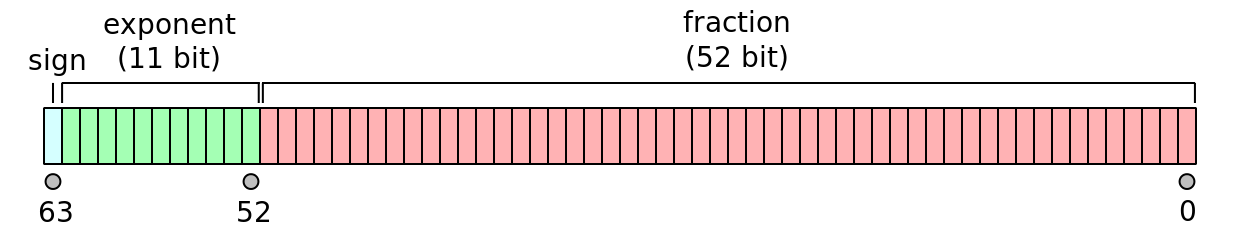
\includegraphics[width=\textwidth]{floating_point_num.png}

Стойността на числото се изчислява по формулата $(-1)^{sign} (1.mantissa) 2^{exp - \lfloor max(exp)/2 \rfloor}$, където $sign = b_{63}, exp = b_{62}b_{61} \dots b_{52}, mantissa = b_{51}b_{50} \dots b_{0}$, $max(exp)$ е максималната стойност на $exp$ (при 64-битови числа е 2046) и $b_i$ е битът на позиция $i$.
\bigbreak
Други особености са, че не е комутативен. Също така е препоръчително при сравнения на рационални променливи да се добавя $\varepsilon \in \mathbb{Q}, \varepsilon > 0$ и $\varepsilon$ достатъчно малък за да не наруши необходимата точност.
\bigbreak
В \textit{C++} рационалните променливи се означават чрез ключовите думи \textit{float} и \textit{double}, като те обичайно заемат съответно по 4b и 8b. Примери за дефиниция са:

\begin{lstlisting}[language=C++, caption=Real numbers]
double a; // undefined default value
double b = 5.0;
\end{lstlisting}

Следните оператори могат да бъдат прилагани над рационални променливи:

\begin{lstlisting}[language=C++, caption=Real number operations]
double a = -1.0, b = 5.0, c = 0.0;

// Unary ops are similar to the ones with integers
-a; +a; // ~1.0, ~-1.0
++a; a++; --a; a--; // ~0.0, ~1.0, ~0.0, ~-1.0

// Arithmetics work similar to the ones with integers
a + b; a - b; // ~4.0, ~-6.0
a / b; a * b; // ~-0.2, ~-5.0
// a % b is not allowed

// Boolean ops
// Numbers different from 0.0 are interpreted as true
a && c; a && b; // 0.0, 1.0
a || c; c || c; // 1.0, 0.0
!c; !!c; // 0.0, 1.0

// Comparison ops are the same as with integers

// IO ops
std::cin >> a; // reads the number from the stdin fd
std::cout << a; // sends the number string represenation to the stdout fd
\end{lstlisting}

\section{Основни структури от данни}
\subsection{Съставни типове от данни}

\noindent \textit{\textbf{Деф}} - Структурите от данни представляват начин за организация на информация с цел по-ефикасното ѝ използване.

\subsection{Структура от данни масив}

\noindent \textit{\textbf{Деф}} - Масивът е крайна редица от фиксиран брой хомогенни елементи, т.е. от един и същи тип, без значение дали е скаларен или съставен.
Всеки елемент е индексиран, което позволява пряк достъп до него.
\bigbreak
Има два вида масиви - статични и динамични, като това се определя по начина, по който паметта се заделя.
Статичните масиви се заделят на стека или в глобалната секция с данни на програмата. И в двата случая размерът им трябва да 
е \textbf{compile time constant}, т.е. известен по време на компилация.
Динамичните масиви използват памет на \textbf{heap}-a, която се заделя по време на изпълнение на програмата.
Това съответно позволява размерът им също да се определя по време на изпълнението.
\bigbreak
Елементите на даден масив се заделят последователно в паметта.
Това позволява конкретен такъв да бъде достъпен директно с индекса си.
Отдолу това се извършва чрез \textbf{pointer arithmetic}, която от своя страна ползва размера на типа в масива.
\bigbreak
В \textit{C++} масив се дефинира чрез типа масив.

\subsection{Тип масив}

Типът масив се определя чрез задаване на типа и броя на елементите на редицата, определяща масив.
Нека \textbf{T} е име или дефиниция на произволен тип, различен от псевдоним, \textbf{void} и функционален, а \textbf{size} е неотрицателна целочислена променлива.
Тогава \textbf{T[size]} е тип масив от \textbf{size} елемента от тип \textbf{T}.
Елементите се индексират от \textbf{0} до \textbf{size–1}.
\textbf{T} се нарича базов тип, а \textbf{size} – размер/капацитет.

Променлива от тип масив се дефинира по начина \textbf{T <arr\_name>[size] [= \{<comma\_separated\_constanst\_values>\}]} или \textbf{T <arr\_name>[] = \{<comma\_separated\_constanst\_values>\}}.
Примери са:

\begin{lstlisting}[language=C++, caption=Example array definitions]
int a[5]; // array with 5 elements of type int indexed from 0 to 4
double b[10]; // array with 5 elements of type double indexed from 0 to 9

bool c[] = {false, true, false, true, true}; // array with 5 elements of type bool
\end{lstlisting}

Множеството от допустими стойности на типа \textbf{T[size]} се състои от всички редици от по \textbf{size} елемента, които са произволни константи от тип \textbf{T}.
Елементите от множеството от допустими стойности на даден тип масив са константите на този тип масив.
\bigbreak
Елементите на масив с размер \textbf{size} са индексирани поледователно с естественитe числа от \textbf{0} до \textbf{size-1}.
Достъпът до конкретен елемент се осъществява посредством неговата индексирана променлива.
Индексираните променливи имат следния синтаксис \textbf{<indexed\_var> := <arr\_name>[index]}, където \textbf{index} е от целочислен тип.
Пример е:

\begin{lstlisting}[language=C++, caption=Example array item access]
int a[] = {1, 2, 85, 4, 101};

a[0]; a[1]; a[2]; a[3]; a[4]; // 1, 2, 85, 4, 101
// a[5]; yields a segfault error
\end{lstlisting}

\section{Тип указател}
\subsection{Дефиниция}
Указателите съдържат \textbf{адреси} към променлива (или променливи) от даден \textbf{тип}.
Същият тип се използва при дефинирането на указателите:

\begin{lstlisting}[language=C++, caption=Pointer example]
int * a = nullptr;
double * b;
char * c;
\end{lstlisting}

Можем да дефинираме и указател към указател - т.е. можем да добавяме произволно много нива на \textbf{indirection}.
\begin{lstlisting}[language=C++, caption=Pointer example]
int ** a = nullptr;
double *** b = 0;
char **** c;
\end{lstlisting}

Напрактика броя на звездичките следва експоненциално разпределение: най-често се ползват просто указатели, след това двойни указатели и т.н.
Ако указателя е към структура или клас, се използва \textbf{->} за достъп до полетата:

\begin{lstlisting}[language=C++, caption=Pointer to struct example]
struct alabala
{
    int ala;
    double bala;
};

alabala ab1;
alabala * pab = &ab1;

pab->ala = 3;
pab->bala = 3.14;
\end{lstlisting}

\subsection{Размер}
Размерът на указателите зависи от големината на адресното пространство. Следователно размерът е 2 (16 битова система), 4 (32 битова), 
или 8 байта (64 битова).

\subsection{Основни операции}
Адрес на променлива можем да извлечем чрез оператора \textbf(\&). Този адрес можем да присвоим на указател. 
Чрез оператора \textbf{*} можем да достъпим и променяме стойността на променливата, към която указателят сочи.
\begin{lstlisting}[language=C++, caption=Pointer example 2]
int a = 5;
int * ptr = &a;
*ptr = 7;
// a is now 7
\end{lstlisting}

Можем да добавяме и изваждаме \textbf{цели} числа от указатели. Това премества указателя да сочи към съседни променливи.
Можем да изваждаме указател от указател, като резултатът от това е \textbf{цяло} число, което показва колко променливи от 
дадения тип има между двата указателя (със знак). Събиране на два указателя е безсмислено.

\begin{lstlisting}[language=C++, caption=Pointer example 3]
int * base_ptr = ...;
int * curr_ptr = base_ptr + i;
int * best_ptr = ...;
int distance = best_ptr - base_ptr;
\end{lstlisting}

Указателите могат да участват в булеви изрази директно. Изразите се оценяват на \textbf{true}, ако указателят не е нулев (0 или \textbf{nullptr}).
Обикновено достъпването на нулев указател води до \textbf{runtime error}.

\subsection{Указателна аритметика}
При гореописаните операции се взима впредвид \textbf{типа} на указателя. При добавяне на число $n$ към указател, който в момента сочи към $a$, се 
добавя $n . sizeof(T)$, където $T$ е типа на указателя. Аналогично, при изваждане на указатели разликата в адресите се дели на размера на типа.

\subsection{Указатели и едномерни масиви}

Указателите имат дефиниран \textbf{operator[]}, който е съкратен запис на \textbf{*} и добавяне на число към указател:
\begin{lstlisting}[language=C++, caption=Pointer example 3]
int * base_ptr = ...;

// These two are equivalent
*(base_ptr + i) = i;
base_ptr[i] = i;
\end{lstlisting}

Всъщност така се имплементира индексирането на масиви. Променливите от тип масив автоматично се конвертират към тип указател.
Единствената разлика е, че няма как типа на указателя да съхранява към колко обекта сочи, т.е.:

\begin{lstlisting}[language=C++, caption=Pointer example 3]
int arr[] = { 1, 2, 3 };
int * p = arr;

int size_1 = sizeof(arr) / sizeof(arr[0]); // 3
int size_2 = sizeof(p) / sizeof(p[0]); // 0, 1 or 2 - depending on how big the pointer is wrt to the int type
\end{lstlisting}

\subsection{Указатели и многомерни масиви}
Адресното пространство е линейно, което означава че многомерните масиви трябва да се записват като един или няколко едномерни.
Начина, по който са записани, се отразява на типа на указателите, които сочат към тях.

\subsubsection{Заделени като един едномерен масив}
В този случай целият масив заема един блок памет. Единствената разлика с едномерен масив е, че са известни всички без първото измерение:
\begin{lstlisting}[language=C++, caption=Multidimensional pointers]
int arr[3][5][7];
int (*)p[5][7] = a;

// These do the same thing
arr[1][1][1] = 1;
p[1][1][1] = 1;
\end{lstlisting}

В случая \textbf{p} сочи към масив от \textbf{5x7 двумерни масиви}. Същия синтаксис можем да ползваме за произволна размерност.
При адресация на отделни елементи, компилатора взема впредвид индивидуалните размери.

Ако многомерният масив не е с предварително известни всички-без-едно-измерения, то този начин на дефиниране на указатели и адресация
не може да работи, защото компилатора няма как да върши сметките вместо нас. В този случай е необходимо ръчно да изчислияваме линейните адреси.
Ще дадем често срещан пример в практиката - триканално \textit{RGB} изображение:
\begin{lstlisting}[language=C++, caption=Multidimensional pointers]
uint8_t * image = ...;

// These may not be compile time constants
int width = 1920;
int height = 1080;
int ch = 3;

int x = 100;
int y = 50;

// Set the green component of the (x, y) to 128
image[y * width * ch + x * ch + 1] = 128;

// Alternatively, first obtain pointer to y-th line of image
int * line_ptr = image + y * width * ch;
line_ptr[x * ch + 1] = 128;
\end{lstlisting}

\subsubsection{Заделени като много едномерни масиви}
В този случай имаме масив от указатели (в двумерния случай). Всеки указател сочи към масив от елементи от съответния тип.
Съответно не е задължително всички подмасиви да са с еднакъв размер, дори не е задължително да няма припокриване.
Следователно е леко спорно доколко това реално са \textit{масиви}, но го споменава, защото това позволява използването
на [] адресацията дори когато размерите не са известни по време на компилация:

\begin{lstlisting}[language=C++, caption=Multidimensional pointers 2]
int ** matrix = ...;
int size = 9;

matrix[3][5] = 17; // OK
matrix[3 * size + 5] = 17; // NOT the same! Probably points to memory we shouldn't touch
\end{lstlisting}

В този случай за достъп до всеки елемент се минава през 2 указателя, докато минаваме само през 1 при предходния подход.

\subsection{Указатели и низове}
Специален клас низове, наречени \textbf{C strings}, се дефинират единствено с указател към символния тип \textbf{char}.
Тези низове винаги завършват с нулев байт, което означава, че няма нужда да се съхранява дължината им.
В стандартана библиотека има много функции, работещи с такива низове: \textit{strlen, strcmp, strcpy, \dots}.

\subsection{Константи указатели и указатели към константа}
Думичката \textbf{const} може да се приложи на няколко места в дефиницията на указател, но има само две различни (но не взаимноизключващи) функции:
\begin{itemize}
    \item Ако \textbf{const} се появи преди \textbf{*}, то указателят е към \textbf{константен тип} $\Rightarrow$ стойността на променливата \textbf{НЕ} може да се променя през него
    \item Ако \textbf{const} се появи след \textbf{*}, то указателят е константен. Това означава, че може да му се присвои стойност единствено при инициализация. След това тя \textbf{не} може да бъде променяна.
\end{itemize}

\begin{lstlisting}[language=C++, caption=Multidimensional pointers 2]
int a = 5;
const int b = 7;

const int * p1 = &a; // OK, a cannot be changed through p1
int const * p2 = &a; // OK, same as p1
int * p3 = & a; // OK, value can be changed through p3

int * p4 = &b; // Compile error, type of p4 says that value of b can be changed through it, but b is const
const int * p5 = &b; // OK, types agree
p5 = &a; // OK, pointer itself is not const

int * const p6 = a; // OK, p6 cannot be redirected
const int * const p7 = b; // OK

p7 = p6; // Error, p7 is a const pointer
\end{lstlisting}

\subsection{Указатели към void}
Възможно е да дефинираме указатели към данни без тип - \textbf{void*}. С тях не може да се извършва аритметика, защото тя изисква размер на тип, 
а при тях тип няма. Естествено, могат да се конвертират към указатели с тип. \textbf{Const} можем да ползваме по нормалния начин.
Този тип указатели се ползват когато не знаем и/или не ни интересува типа на данните. Пример: имаме \textit{C++} библиотека, работеща с класове,
но искаме да направим \textit{C} интерфейс. При \textit{C} класове няма, следователно няма как да сложим указатели с тип конкретните класове
в интерфейсните функции. Можем вместо това да сложим указатели \textbf{void*}, с които \textit{C} може да работи. Вътре в тялото на функцията
конвертираме до указател към съответният клас и работим с него.

\subsection{Псевдоними}
\label{references}
Псевдонимите са като константите указатели, с няколко разлики:
\begin{itemize}
    \item Не участват в адресна аритметика
    \item Сочат към точно един елемент - не може да се използват за достъп до съседни. Не могат да сочат към нищо.
    \item Не се използва \textbf{*} за достъп до стойността
    \item Когато псевдонима е към клас или структура, се използва \textbf{.} вместо \textbf{->} за достъп до индивидуалните полета
\end{itemize}

\begin{lstlisting}[language=C++, caption=Pointer example 2]
int a = 5;
int & ra = a;
ra = 7;
// a is now 7
\end{lstlisting}

\section{Функции}
\subsection{Дефиниране на функция}
Функциите представлят блокове код, които се преизползват. Всяка функция приема параметри (може и 0),
заделя памет за локални параметри и връща резултат (може и да е \textbf{void}, т.е. няма резултат)
при всяко обръщение.

Функциите в \textit{C++} се състоят от две части: \textbf{декларация} и \textbf{дефиниция}.
И двете започват по един и същ начин: \textbf{<return type> <function name>(<parameter list>)}.
При декларацията редът завършва с \textbf{;}, а при дефиницията - отваря се блок с \textbf{\{}, 
в който се пише кодът на функцията. Декларациите казват на компилатора \textit{такава функция съществува},
а дефинициите казват \textit{такава функция съществува и това е кодът й}.

Всяка от двете части е \textit{незадължителна}. Можем да използваме само \textbf{декларации}, ако функцията е 
дефинирана на друго място (друг \textbf{.cpp} файл, външна библиотека). Ако такова друго място не съществува, 
получаваме грешка при свързаването (\textbf{linker error}).

Можем да използваме само \textbf{дефиниция}, ако ще изпозлваме функцията \textbf{след} дефиницията в рамките на същия \textbf{translation unit} (файл).
Ако се опитаме да я ползваме на друго място, получаваме грешка при компилация.

Декларация и дефиниция трябва да съвпадат. Единственото изключение са \textbf{параметрите по избор}, които се задават само 
в декларацията, ако я има.

Можем да добавим и допълнителни атрибути на функция при декларация и дефиниция:
\begin{itemize}
    \item \textbf{static} - означава, че функцията е видима само за текущия \textbf{translation unit}. Код от други места не я вижда, дори да сме добавили декларация.
    \item \textbf{inline} - \textit{подсказка} към компилатора, че тази функция е добре да се вгради директно на всяко място, където се вика. Дали 
    функцията реално се вгражда зависи от компилатора - понякога се гражда дори без \textbf{inline}, понякога не се вгражда дори с \textbf{inline}.
    \item тип на извикването - къде да се записват параметрите (регистри, стек), кой за какво е отговорен да запази. Примери: \textbf{stdcall}, \textbf{fastcall}, \textbf{cdecl}
    \item специфични опции на компилатора
\end{itemize}

\subsection{Обръщение към функция}
Можем да се обръщаме към функция чрез името й. Ако списъка с параметри не е празен, то трябва да подадем правилния тип параметри на правилните места.
Ако функцията връща резултат, можем да го присвоим на променлива от същия, или съвместим, тип.

\subsection{Предаване на параметрите по стойност}
При подаването на параметри по стойност всеки параметър се \textbf{копира}, т.е. функцията получава свое локално копие. 
Дори да го модифицира, това не се отразява в кода, който е направил обращението. Подаването по стойност е подходящо за примитивни и 
\textit{малки} съставни типове. Трябва да се избягва за големи типове, защото е неефикасно и най-вероятно е бъг.

\subsection{Предаване на параметрите чрез указател}
Подаването чрез указател е същото като по стойност, с разликата че се копира указателят, а не стойността, към която сочи.
Това позволява на функцията да променя стойността на параметъра. Предаването чрез указател е подходящо за масиви, за които 
измеренията не са ясни по време на компилация. Също така могат да се използват за параметри, които е позволено да са празни, т.е.
да имаме \textbf{nullptr}.

\subsection{Предаване на параметрите чрез псевдоним}
Както вече казахме в \ref{references}, псевдонимите функционират като ограничени константни указатели.
Подходящи са за подаване на сложни типове, които не могат да са празни. Ако параметърът няма да се променя от функцията,
е добра практика да се ползва \textbf{const}.

\subsection{Масиви като формални параметри}
Ако искаме функцията да работи с многомерни масиви с известни измерения (всички без първото), то можем да зададем това в декларацията и/или дефиницията:
\begin{lstlisting}[language=C++, caption=Arrays as arguments]
int do_3d_stuff(int arr[][3][7], const int size)
{
    ...
}
\end{lstlisting}

Дори да споменем първото измерение, компилатора ще го игнорира и ще позволява функцията да бъде извиквана от масиви със същите последни, 
но различно първо измерение. Ако не знаем предварително всички без първото измерение, тогава трябва да подадем масива чрез указател, 
както и отделните размери в отделни параметри.

\end{document}
